\documentclass[twoside]{book}

% Packages required by doxygen
\usepackage{fixltx2e}
\usepackage{calc}
\usepackage{doxygen}
\usepackage[export]{adjustbox} % also loads graphicx
\usepackage{graphicx}
\usepackage[utf8]{inputenc}
\usepackage{makeidx}
\usepackage{multicol}
\usepackage{multirow}
\PassOptionsToPackage{warn}{textcomp}
\usepackage{textcomp}
\usepackage[nointegrals]{wasysym}
\usepackage[table]{xcolor}

% Font selection
\usepackage[T1]{fontenc}
\usepackage[scaled=.90]{helvet}
\usepackage{courier}
\usepackage{amssymb}
\usepackage{sectsty}
\renewcommand{\familydefault}{\sfdefault}
\allsectionsfont{%
  \fontseries{bc}\selectfont%
  \color{darkgray}%
}
\renewcommand{\DoxyLabelFont}{%
  \fontseries{bc}\selectfont%
  \color{darkgray}%
}
\newcommand{\+}{\discretionary{\mbox{\scriptsize$\hookleftarrow$}}{}{}}

% Page & text layout
\usepackage{geometry}
\geometry{%
  a4paper,%
  top=2.5cm,%
  bottom=2.5cm,%
  left=2.5cm,%
  right=2.5cm%
}
\tolerance=750
\hfuzz=15pt
\hbadness=750
\setlength{\emergencystretch}{15pt}
\setlength{\parindent}{0cm}
\setlength{\parskip}{3ex plus 2ex minus 2ex}
\makeatletter
\renewcommand{\paragraph}{%
  \@startsection{paragraph}{4}{0ex}{-1.0ex}{1.0ex}{%
    \normalfont\normalsize\bfseries\SS@parafont%
  }%
}
\renewcommand{\subparagraph}{%
  \@startsection{subparagraph}{5}{0ex}{-1.0ex}{1.0ex}{%
    \normalfont\normalsize\bfseries\SS@subparafont%
  }%
}
\makeatother

% Headers & footers
\usepackage{fancyhdr}
\pagestyle{fancyplain}
\fancyhead[LE]{\fancyplain{}{\bfseries\thepage}}
\fancyhead[CE]{\fancyplain{}{}}
\fancyhead[RE]{\fancyplain{}{\bfseries\leftmark}}
\fancyhead[LO]{\fancyplain{}{\bfseries\rightmark}}
\fancyhead[CO]{\fancyplain{}{}}
\fancyhead[RO]{\fancyplain{}{\bfseries\thepage}}
\fancyfoot[LE]{\fancyplain{}{}}
\fancyfoot[CE]{\fancyplain{}{}}
\fancyfoot[RE]{\fancyplain{}{\bfseries\scriptsize Generated by Doxygen }}
\fancyfoot[LO]{\fancyplain{}{\bfseries\scriptsize Generated by Doxygen }}
\fancyfoot[CO]{\fancyplain{}{}}
\fancyfoot[RO]{\fancyplain{}{}}
\renewcommand{\footrulewidth}{0.4pt}
\renewcommand{\chaptermark}[1]{%
  \markboth{#1}{}%
}
\renewcommand{\sectionmark}[1]{%
  \markright{\thesection\ #1}%
}

% Indices & bibliography
\usepackage{natbib}
\usepackage[titles]{tocloft}
\setcounter{tocdepth}{3}
\setcounter{secnumdepth}{5}
\makeindex

% Hyperlinks (required, but should be loaded last)
\usepackage{ifpdf}
\ifpdf
  \usepackage[pdftex,pagebackref=true]{hyperref}
\else
  \usepackage[ps2pdf,pagebackref=true]{hyperref}
\fi
\hypersetup{%
  colorlinks=true,%
  linkcolor=blue,%
  citecolor=blue,%
  unicode%
}

% Custom commands
\newcommand{\clearemptydoublepage}{%
  \newpage{\pagestyle{empty}\cleardoublepage}%
}

\usepackage{caption}
\captionsetup{labelsep=space,justification=centering,font={bf},singlelinecheck=off,skip=4pt,position=top}

%===== C O N T E N T S =====

\begin{document}

% Titlepage & ToC
\hypersetup{pageanchor=false,
             bookmarksnumbered=true,
             pdfencoding=unicode
            }
\pagenumbering{roman}
\begin{titlepage}
\vspace*{7cm}
\begin{center}%
{\Large My Project }\\
\vspace*{1cm}
{\large Generated by Doxygen 1.8.11}\\
\end{center}
\end{titlepage}
\clearemptydoublepage
\tableofcontents
\clearemptydoublepage
\pagenumbering{arabic}
\hypersetup{pageanchor=true}

%--- Begin generated contents ---
\chapter{Namespace Index}
\section{Namespace List}
Here is a list of all namespaces with brief descriptions\+:\begin{DoxyCompactList}
\item\contentsline{section}{\hyperlink{namespacequeuesavitch}{queuesavitch} }{\pageref{namespacequeuesavitch}}{}
\end{DoxyCompactList}

\chapter{Hierarchical Index}
\section{Class Hierarchy}
This inheritance list is sorted roughly, but not completely, alphabetically\+:\begin{DoxyCompactList}
\item \contentsline{section}{Fruit}{\pageref{classFruit}}{}
\begin{DoxyCompactList}
\item \contentsline{section}{Apple}{\pageref{classApple}}{}
\item \contentsline{section}{Grape}{\pageref{classGrape}}{}
\item \contentsline{section}{Orange}{\pageref{classOrange}}{}
\end{DoxyCompactList}
\item \contentsline{section}{List}{\pageref{classList}}{}
\item \contentsline{section}{List\+:\+:Node}{\pageref{structList_1_1Node}}{}
\end{DoxyCompactList}

\chapter{Class Index}
\section{Class List}
Here are the classes, structs, unions and interfaces with brief descriptions\+:\begin{DoxyCompactList}
\item\contentsline{section}{\hyperlink{structnode}{node} }{\pageref{structnode}}{}
\item\contentsline{section}{\hyperlink{structnode1}{node1} }{\pageref{structnode1}}{}
\item\contentsline{section}{\hyperlink{structnode__info}{node\+\_\+info} }{\pageref{structnode__info}}{}
\end{DoxyCompactList}

\chapter{File Index}
\section{File List}
Here is a list of all files with brief descriptions\+:\begin{DoxyCompactList}
\item\contentsline{section}{\hyperlink{Lab1_8c}{Lab1.\+c} }{\pageref{Lab1_8c}}{}
\end{DoxyCompactList}

\chapter{Namespace Documentation}
\hypertarget{namespacequeuesavitch}{}\section{queuesavitch Namespace Reference}
\label{namespacequeuesavitch}\index{queuesavitch@{queuesavitch}}
\subsection*{Classes}
\begin{DoxyCompactItemize}
\item 
class \hyperlink{classqueuesavitch_1_1PriorityQueue}{Priority\+Queue}
\item 
class \hyperlink{classqueuesavitch_1_1Queue}{Queue}
\item 
struct \hyperlink{structqueuesavitch_1_1QueueNode}{Queue\+Node}
\end{DoxyCompactItemize}
\subsection*{Typedefs}
\begin{DoxyCompactItemize}
\item 
typedef \hyperlink{structqueuesavitch_1_1QueueNode}{Queue\+Node} $\ast$ \hyperlink{namespacequeuesavitch_a3a9d48cafb7ea2049936da3b05a10209}{Queue\+Node\+Ptr}
\end{DoxyCompactItemize}


\subsection{Typedef Documentation}
\index{queuesavitch@{queuesavitch}!Queue\+Node\+Ptr@{Queue\+Node\+Ptr}}
\index{Queue\+Node\+Ptr@{Queue\+Node\+Ptr}!queuesavitch@{queuesavitch}}
\subsubsection[{\texorpdfstring{Queue\+Node\+Ptr}{QueueNodePtr}}]{\setlength{\rightskip}{0pt plus 5cm}typedef {\bf Queue\+Node}$\ast$ {\bf queuesavitch\+::\+Queue\+Node\+Ptr}}\hypertarget{namespacequeuesavitch_a3a9d48cafb7ea2049936da3b05a10209}{}\label{namespacequeuesavitch_a3a9d48cafb7ea2049936da3b05a10209}

\chapter{Class Documentation}
\hypertarget{classqueuesavitch_1_1PriorityQueue}{}\section{queuesavitch\+:\+:Priority\+Queue Class Reference}
\label{classqueuesavitch_1_1PriorityQueue}\index{queuesavitch\+::\+Priority\+Queue@{queuesavitch\+::\+Priority\+Queue}}


{\ttfamily \#include $<$Priority\+Queue.\+h$>$}



Inheritance diagram for queuesavitch\+:\+:Priority\+Queue\+:
\nopagebreak
\begin{figure}[H]
\begin{center}
\leavevmode
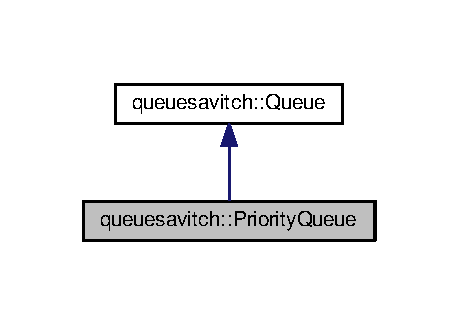
\includegraphics[width=220pt]{classqueuesavitch_1_1PriorityQueue__inherit__graph}
\end{center}
\end{figure}


Collaboration diagram for queuesavitch\+:\+:Priority\+Queue\+:
\nopagebreak
\begin{figure}[H]
\begin{center}
\leavevmode
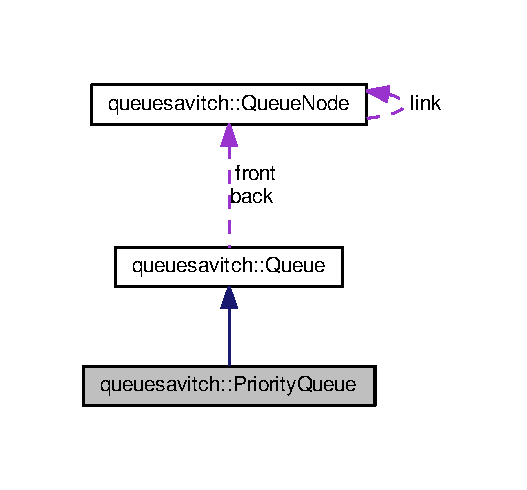
\includegraphics[width=253pt]{classqueuesavitch_1_1PriorityQueue__coll__graph}
\end{center}
\end{figure}
\subsection*{Public Member Functions}
\begin{DoxyCompactItemize}
\item 
\hyperlink{classqueuesavitch_1_1PriorityQueue_a3c599b47f8d383b0be9f74f741331e5e}{Priority\+Queue} ()
\item 
\hyperlink{classqueuesavitch_1_1PriorityQueue_a4ada9c3a90e3a05d9be0b93a486b3fd6}{Priority\+Queue} (const \hyperlink{classqueuesavitch_1_1PriorityQueue}{Priority\+Queue} \&a\+P\+Queue)
\item 
\hyperlink{classqueuesavitch_1_1PriorityQueue_adcefa02407d1df4f9e111bc0ecca81cc}{$\sim$\+Priority\+Queue} ()
\item 
int \hyperlink{classqueuesavitch_1_1PriorityQueue_aabec9a46c41b0601f05f55a7894d20e1}{remove} ()
\end{DoxyCompactItemize}
\subsection*{Additional Inherited Members}


\subsection{Constructor \& Destructor Documentation}
\index{queuesavitch\+::\+Priority\+Queue@{queuesavitch\+::\+Priority\+Queue}!Priority\+Queue@{Priority\+Queue}}
\index{Priority\+Queue@{Priority\+Queue}!queuesavitch\+::\+Priority\+Queue@{queuesavitch\+::\+Priority\+Queue}}
\subsubsection[{\texorpdfstring{Priority\+Queue()}{PriorityQueue()}}]{\setlength{\rightskip}{0pt plus 5cm}queuesavitch\+::\+Priority\+Queue\+::\+Priority\+Queue (
\begin{DoxyParamCaption}
{}
\end{DoxyParamCaption}
)}\hypertarget{classqueuesavitch_1_1PriorityQueue_a3c599b47f8d383b0be9f74f741331e5e}{}\label{classqueuesavitch_1_1PriorityQueue_a3c599b47f8d383b0be9f74f741331e5e}

\begin{DoxyCode}
16                                 : \hyperlink{classqueuesavitch_1_1Queue_a76c2a8339bb4ab4f22f0f425be154c6a}{Queue}()
17    \{
18       \textcolor{comment}{//Intentionally empty.                                                                               
                                                                                                       }
19    \}
\end{DoxyCode}
\index{queuesavitch\+::\+Priority\+Queue@{queuesavitch\+::\+Priority\+Queue}!Priority\+Queue@{Priority\+Queue}}
\index{Priority\+Queue@{Priority\+Queue}!queuesavitch\+::\+Priority\+Queue@{queuesavitch\+::\+Priority\+Queue}}
\subsubsection[{\texorpdfstring{Priority\+Queue(const Priority\+Queue \&a\+P\+Queue)}{PriorityQueue(const PriorityQueue &aPQueue)}}]{\setlength{\rightskip}{0pt plus 5cm}queuesavitch\+::\+Priority\+Queue\+::\+Priority\+Queue (
\begin{DoxyParamCaption}
\item[{const {\bf Priority\+Queue} \&}]{a\+P\+Queue}
\end{DoxyParamCaption}
)}\hypertarget{classqueuesavitch_1_1PriorityQueue_a4ada9c3a90e3a05d9be0b93a486b3fd6}{}\label{classqueuesavitch_1_1PriorityQueue_a4ada9c3a90e3a05d9be0b93a486b3fd6}

\begin{DoxyCode}
22    \{
23       \hyperlink{classqueuesavitch_1_1Queue_ac30555d398c28ad9b72f9d9b05c1ddf6}{front} = aPQueue.front;
24       \hyperlink{classqueuesavitch_1_1Queue_a2759a808c5c9abe7d1c53cc8ade3f5a9}{back} = aPQueue.back;
25       \textcolor{comment}{// Self-test exercise 12                                                                             
                                                                                                       }
26    \}
\end{DoxyCode}
\index{queuesavitch\+::\+Priority\+Queue@{queuesavitch\+::\+Priority\+Queue}!````~Priority\+Queue@{$\sim$\+Priority\+Queue}}
\index{````~Priority\+Queue@{$\sim$\+Priority\+Queue}!queuesavitch\+::\+Priority\+Queue@{queuesavitch\+::\+Priority\+Queue}}
\subsubsection[{\texorpdfstring{$\sim$\+Priority\+Queue()}{~PriorityQueue()}}]{\setlength{\rightskip}{0pt plus 5cm}queuesavitch\+::\+Priority\+Queue\+::$\sim$\+Priority\+Queue (
\begin{DoxyParamCaption}
{}
\end{DoxyParamCaption}
)}\hypertarget{classqueuesavitch_1_1PriorityQueue_adcefa02407d1df4f9e111bc0ecca81cc}{}\label{classqueuesavitch_1_1PriorityQueue_adcefa02407d1df4f9e111bc0ecca81cc}

\begin{DoxyCode}
29    \{
30       \textcolor{comment}{//The definition of the destructor is Self-Test Exercise 13.                                         
                                                                                                       }
31    \}
\end{DoxyCode}


\subsection{Member Function Documentation}
\index{queuesavitch\+::\+Priority\+Queue@{queuesavitch\+::\+Priority\+Queue}!remove@{remove}}
\index{remove@{remove}!queuesavitch\+::\+Priority\+Queue@{queuesavitch\+::\+Priority\+Queue}}
\subsubsection[{\texorpdfstring{remove()}{remove()}}]{\setlength{\rightskip}{0pt plus 5cm}int queuesavitch\+::\+Priority\+Queue\+::remove (
\begin{DoxyParamCaption}
{}
\end{DoxyParamCaption}
)\hspace{0.3cm}{\ttfamily [virtual]}}\hypertarget{classqueuesavitch_1_1PriorityQueue_aabec9a46c41b0601f05f55a7894d20e1}{}\label{classqueuesavitch_1_1PriorityQueue_aabec9a46c41b0601f05f55a7894d20e1}


Reimplemented from \hyperlink{classqueuesavitch_1_1Queue_a607e9543f593526aee0d6a403a4ce775}{queuesavitch\+::\+Queue}.


\begin{DoxyCode}
35    \{
36       \textcolor{keywordflow}{if} (\hyperlink{classqueuesavitch_1_1Queue_a557c2aefa6d1c51d42a1563dab0e2cc0}{empty}())
37       \{
38          cout << \textcolor{stringliteral}{"Error: Removing an item from an empty queue.\(\backslash\)n"};
39          exit(1);
40       \}
41       \hyperlink{namespacequeuesavitch_a3a9d48cafb7ea2049936da3b05a10209}{QueueNodePtr} p = \hyperlink{classqueuesavitch_1_1Queue_ac30555d398c28ad9b72f9d9b05c1ddf6}{front};
42       \hyperlink{namespacequeuesavitch_a3a9d48cafb7ea2049936da3b05a10209}{QueueNodePtr} discard, previous, here;
43       \hyperlink{namespacequeuesavitch_a3a9d48cafb7ea2049936da3b05a10209}{QueueNodePtr} next;
44       \textcolor{keywordtype}{int} target = \hyperlink{classqueuesavitch_1_1Queue_ac30555d398c28ad9b72f9d9b05c1ddf6}{front}->\hyperlink{structqueuesavitch_1_1QueueNode_a4fd17a591c8510ed1118d3c4cb67b320}{data};
45       \textcolor{keywordflow}{while}(p->link != NULL)
46       \{
47          here = p->link;
48          \textcolor{keywordflow}{if}(here->data < target) \textcolor{comment}{// if a node has a value smaller than the first node's                    
                                                                                                       }
49          \{
50             target = here->data;
51             discard = here;
52             previous = p;
53          \}
54          p = p->link;
55       \}
56 
57       \textcolor{keywordflow}{if}(target == \hyperlink{classqueuesavitch_1_1Queue_ac30555d398c28ad9b72f9d9b05c1ddf6}{front}->\hyperlink{structqueuesavitch_1_1QueueNode_a4fd17a591c8510ed1118d3c4cb67b320}{data}) \textcolor{comment}{// if the first node holds the smallest value                     
                                                                                                                }
58       \{
59          discard = \hyperlink{classqueuesavitch_1_1Queue_ac30555d398c28ad9b72f9d9b05c1ddf6}{front};
60         \hyperlink{classqueuesavitch_1_1Queue_ac30555d398c28ad9b72f9d9b05c1ddf6}{front} = \hyperlink{classqueuesavitch_1_1Queue_ac30555d398c28ad9b72f9d9b05c1ddf6}{front}->\hyperlink{structqueuesavitch_1_1QueueNode_add6ebeca47fc7ab55c99a33827cb68c4}{link};
61       \}
62       \textcolor{keywordflow}{else} \textcolor{keywordflow}{if}(discard->link == NULL) \textcolor{comment}{// if the last node holds the smallest value                          
                                                                                                       }
63          \hyperlink{classqueuesavitch_1_1Queue_a2759a808c5c9abe7d1c53cc8ade3f5a9}{back} = previous;
64       \textcolor{keywordflow}{else} \textcolor{comment}{// if a middle node holds the smallest value                                                    
                                                                                                       }
65          previous->\hyperlink{structqueuesavitch_1_1QueueNode_add6ebeca47fc7ab55c99a33827cb68c4}{link} = discard->\hyperlink{structqueuesavitch_1_1QueueNode_add6ebeca47fc7ab55c99a33827cb68c4}{link};
66       \textcolor{keywordflow}{if} (\hyperlink{classqueuesavitch_1_1Queue_ac30555d398c28ad9b72f9d9b05c1ddf6}{front} == NULL) \textcolor{comment}{//if you removed the last node                                               
                                                                                                            }
67          \hyperlink{classqueuesavitch_1_1Queue_a2759a808c5c9abe7d1c53cc8ade3f5a9}{back} = NULL;
68 
69       \textcolor{keyword}{delete} discard;
70 
71       \textcolor{keywordflow}{return} target;
72    \}
\end{DoxyCode}


Here is the call graph for this function\+:
\nopagebreak
\begin{figure}[H]
\begin{center}
\leavevmode
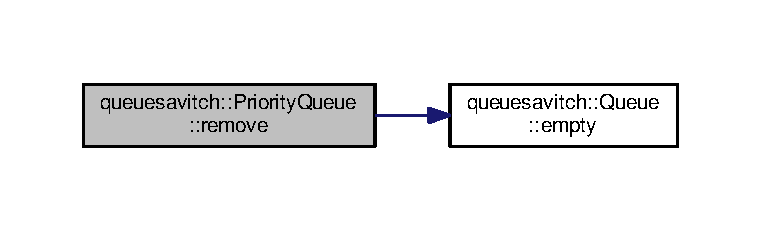
\includegraphics[width=350pt]{classqueuesavitch_1_1PriorityQueue_aabec9a46c41b0601f05f55a7894d20e1_cgraph}
\end{center}
\end{figure}




The documentation for this class was generated from the following files\+:\begin{DoxyCompactItemize}
\item 
\hyperlink{PriorityQueue_8h}{Priority\+Queue.\+h}\item 
\hyperlink{PriorityQueue_8cpp}{Priority\+Queue.\+cpp}\end{DoxyCompactItemize}

\hypertarget{classqueuesavitch_1_1Queue}{}\section{queuesavitch\+:\+:Queue Class Reference}
\label{classqueuesavitch_1_1Queue}\index{queuesavitch\+::\+Queue@{queuesavitch\+::\+Queue}}


{\ttfamily \#include $<$Queue.\+h$>$}



Inheritance diagram for queuesavitch\+:\+:Queue\+:
\nopagebreak
\begin{figure}[H]
\begin{center}
\leavevmode
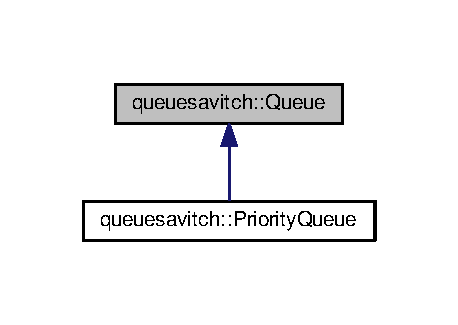
\includegraphics[width=220pt]{classqueuesavitch_1_1Queue__inherit__graph}
\end{center}
\end{figure}


Collaboration diagram for queuesavitch\+:\+:Queue\+:
\nopagebreak
\begin{figure}[H]
\begin{center}
\leavevmode
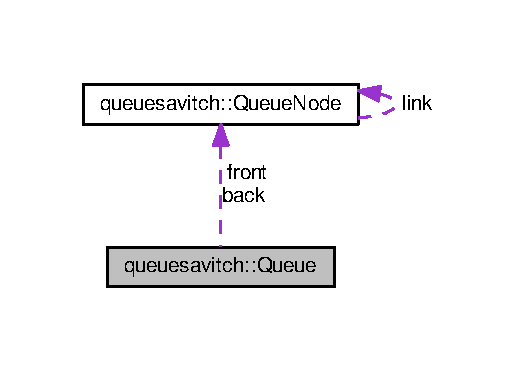
\includegraphics[width=249pt]{classqueuesavitch_1_1Queue__coll__graph}
\end{center}
\end{figure}
\subsection*{Public Member Functions}
\begin{DoxyCompactItemize}
\item 
\hyperlink{classqueuesavitch_1_1Queue_a76c2a8339bb4ab4f22f0f425be154c6a}{Queue} ()
\item 
\hyperlink{classqueuesavitch_1_1Queue_a1ed5fcbcbdbae93132f03c698dd24e8d}{Queue} (const \hyperlink{classqueuesavitch_1_1Queue}{Queue} \&a\+Queue)
\item 
\hyperlink{classqueuesavitch_1_1Queue_a4207b8d35aec9740a04da0953568296f}{$\sim$\+Queue} ()
\item 
void \hyperlink{classqueuesavitch_1_1Queue_a5f208f5455b566a5ddf3bb4a7869cb31}{add} (int item)
\item 
virtual int \hyperlink{classqueuesavitch_1_1Queue_a607e9543f593526aee0d6a403a4ce775}{remove} ()
\item 
bool \hyperlink{classqueuesavitch_1_1Queue_a557c2aefa6d1c51d42a1563dab0e2cc0}{empty} () const 
\end{DoxyCompactItemize}
\subsection*{Protected Attributes}
\begin{DoxyCompactItemize}
\item 
\hyperlink{namespacequeuesavitch_a3a9d48cafb7ea2049936da3b05a10209}{Queue\+Node\+Ptr} \hyperlink{classqueuesavitch_1_1Queue_ac30555d398c28ad9b72f9d9b05c1ddf6}{front}
\item 
\hyperlink{namespacequeuesavitch_a3a9d48cafb7ea2049936da3b05a10209}{Queue\+Node\+Ptr} \hyperlink{classqueuesavitch_1_1Queue_a2759a808c5c9abe7d1c53cc8ade3f5a9}{back}
\end{DoxyCompactItemize}


\subsection{Constructor \& Destructor Documentation}
\index{queuesavitch\+::\+Queue@{queuesavitch\+::\+Queue}!Queue@{Queue}}
\index{Queue@{Queue}!queuesavitch\+::\+Queue@{queuesavitch\+::\+Queue}}
\subsubsection[{\texorpdfstring{Queue()}{Queue()}}]{\setlength{\rightskip}{0pt plus 5cm}queuesavitch\+::\+Queue\+::\+Queue (
\begin{DoxyParamCaption}
{}
\end{DoxyParamCaption}
)}\hypertarget{classqueuesavitch_1_1Queue_a76c2a8339bb4ab4f22f0f425be154c6a}{}\label{classqueuesavitch_1_1Queue_a76c2a8339bb4ab4f22f0f425be154c6a}

\begin{DoxyCode}
19                  : \hyperlink{classqueuesavitch_1_1Queue_ac30555d398c28ad9b72f9d9b05c1ddf6}{front}(NULL), \hyperlink{classqueuesavitch_1_1Queue_a2759a808c5c9abe7d1c53cc8ade3f5a9}{back}(NULL)
20    \{
21       \textcolor{comment}{//Intentionally empty.                                                                               
                                                                                                       }
22    \}
\end{DoxyCode}
\index{queuesavitch\+::\+Queue@{queuesavitch\+::\+Queue}!Queue@{Queue}}
\index{Queue@{Queue}!queuesavitch\+::\+Queue@{queuesavitch\+::\+Queue}}
\subsubsection[{\texorpdfstring{Queue(const Queue \&a\+Queue)}{Queue(const Queue &aQueue)}}]{\setlength{\rightskip}{0pt plus 5cm}queuesavitch\+::\+Queue\+::\+Queue (
\begin{DoxyParamCaption}
\item[{const {\bf Queue} \&}]{a\+Queue}
\end{DoxyParamCaption}
)}\hypertarget{classqueuesavitch_1_1Queue_a1ed5fcbcbdbae93132f03c698dd24e8d}{}\label{classqueuesavitch_1_1Queue_a1ed5fcbcbdbae93132f03c698dd24e8d}

\begin{DoxyCode}
25    \{
26       \hyperlink{classqueuesavitch_1_1Queue_ac30555d398c28ad9b72f9d9b05c1ddf6}{front} = aQueue.front;
27       \hyperlink{classqueuesavitch_1_1Queue_a2759a808c5c9abe7d1c53cc8ade3f5a9}{back} = aQueue.back;
28    \}
\end{DoxyCode}
\index{queuesavitch\+::\+Queue@{queuesavitch\+::\+Queue}!````~Queue@{$\sim$\+Queue}}
\index{````~Queue@{$\sim$\+Queue}!queuesavitch\+::\+Queue@{queuesavitch\+::\+Queue}}
\subsubsection[{\texorpdfstring{$\sim$\+Queue()}{~Queue()}}]{\setlength{\rightskip}{0pt plus 5cm}queuesavitch\+::\+Queue\+::$\sim$\+Queue (
\begin{DoxyParamCaption}
{}
\end{DoxyParamCaption}
)}\hypertarget{classqueuesavitch_1_1Queue_a4207b8d35aec9740a04da0953568296f}{}\label{classqueuesavitch_1_1Queue_a4207b8d35aec9740a04da0953568296f}

\begin{DoxyCode}
32    \{
33       \textcolor{comment}{/*if(front != NULL)                                                                                  
                                                                                                       }
34 \textcolor{comment}{      \{                                                                                                    
                                                                                                       }
35 \textcolor{comment}{         QueueNodePtr here = front;                                                                        
                                                                                                       }
36 \textcolor{comment}{         QueueNodePtr discard;                                                                             
                                                                                                       }
37 \textcolor{comment}{         while(here->link != NULL)                                                                         
                                                                                                       }
38 \textcolor{comment}{         \{                                                                                                 
                                                                                                       }
39 \textcolor{comment}{            discard = here;                                                                                
                                                                                                       }
40 \textcolor{comment}{            here = here->link;                                                                             
                                                                                                       }
41 \textcolor{comment}{            delete discard;                                                                                
                                                                                                       }
42 \textcolor{comment}{         \}                                                                                                 
                                                                                                       }
43 \textcolor{comment}{         \}*/}
44    \}
\end{DoxyCode}


\subsection{Member Function Documentation}
\index{queuesavitch\+::\+Queue@{queuesavitch\+::\+Queue}!add@{add}}
\index{add@{add}!queuesavitch\+::\+Queue@{queuesavitch\+::\+Queue}}
\subsubsection[{\texorpdfstring{add(int item)}{add(int item)}}]{\setlength{\rightskip}{0pt plus 5cm}void queuesavitch\+::\+Queue\+::add (
\begin{DoxyParamCaption}
\item[{int}]{item}
\end{DoxyParamCaption}
)}\hypertarget{classqueuesavitch_1_1Queue_a5f208f5455b566a5ddf3bb4a7869cb31}{}\label{classqueuesavitch_1_1Queue_a5f208f5455b566a5ddf3bb4a7869cb31}

\begin{DoxyCode}
55    \{
56       \textcolor{keywordflow}{if} (\hyperlink{classqueuesavitch_1_1Queue_a557c2aefa6d1c51d42a1563dab0e2cc0}{empty}( ))
57       \{
58          \hyperlink{classqueuesavitch_1_1Queue_ac30555d398c28ad9b72f9d9b05c1ddf6}{front} = \textcolor{keyword}{new} QueueNode;
59          \hyperlink{classqueuesavitch_1_1Queue_ac30555d398c28ad9b72f9d9b05c1ddf6}{front}->\hyperlink{structqueuesavitch_1_1QueueNode_a4fd17a591c8510ed1118d3c4cb67b320}{data} = item;
60        \hyperlink{classqueuesavitch_1_1Queue_a2759a808c5c9abe7d1c53cc8ade3f5a9}{back} = \hyperlink{classqueuesavitch_1_1Queue_ac30555d398c28ad9b72f9d9b05c1ddf6}{front};
61       \}
62 
63       \textcolor{keywordflow}{else}
64       \{
65          \hyperlink{namespacequeuesavitch_a3a9d48cafb7ea2049936da3b05a10209}{QueueNodePtr} temp\_ptr;
66          temp\_ptr = \textcolor{keyword}{new} QueueNode;
67 
68          temp\_ptr->\hyperlink{structqueuesavitch_1_1QueueNode_a4fd17a591c8510ed1118d3c4cb67b320}{data} = item;
69          temp\_ptr->link = NULL;
70          \hyperlink{classqueuesavitch_1_1Queue_a2759a808c5c9abe7d1c53cc8ade3f5a9}{back}->\hyperlink{structqueuesavitch_1_1QueueNode_add6ebeca47fc7ab55c99a33827cb68c4}{link} = temp\_ptr;
71          \hyperlink{classqueuesavitch_1_1Queue_a2759a808c5c9abe7d1c53cc8ade3f5a9}{back} = temp\_ptr;
72       \}
73    \}
\end{DoxyCode}


Here is the call graph for this function\+:
\nopagebreak
\begin{figure}[H]
\begin{center}
\leavevmode
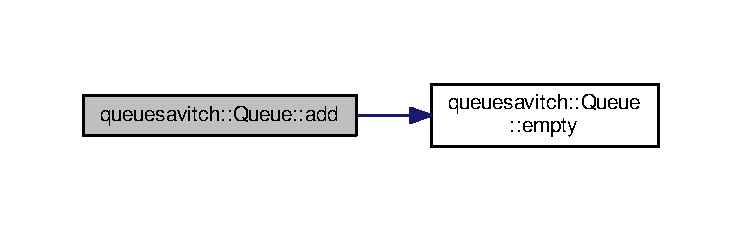
\includegraphics[width=350pt]{classqueuesavitch_1_1Queue_a5f208f5455b566a5ddf3bb4a7869cb31_cgraph}
\end{center}
\end{figure}


\index{queuesavitch\+::\+Queue@{queuesavitch\+::\+Queue}!empty@{empty}}
\index{empty@{empty}!queuesavitch\+::\+Queue@{queuesavitch\+::\+Queue}}
\subsubsection[{\texorpdfstring{empty() const }{empty() const }}]{\setlength{\rightskip}{0pt plus 5cm}bool queuesavitch\+::\+Queue\+::empty (
\begin{DoxyParamCaption}
{}
\end{DoxyParamCaption}
) const}\hypertarget{classqueuesavitch_1_1Queue_a557c2aefa6d1c51d42a1563dab0e2cc0}{}\label{classqueuesavitch_1_1Queue_a557c2aefa6d1c51d42a1563dab0e2cc0}

\begin{DoxyCode}
49    \{
50       \textcolor{keywordflow}{return} (\hyperlink{classqueuesavitch_1_1Queue_a2759a808c5c9abe7d1c53cc8ade3f5a9}{back} == NULL);\textcolor{comment}{//front == NULL would also work                                            
                                                                                                           }
51    \}
\end{DoxyCode}
\index{queuesavitch\+::\+Queue@{queuesavitch\+::\+Queue}!remove@{remove}}
\index{remove@{remove}!queuesavitch\+::\+Queue@{queuesavitch\+::\+Queue}}
\subsubsection[{\texorpdfstring{remove()}{remove()}}]{\setlength{\rightskip}{0pt plus 5cm}int queuesavitch\+::\+Queue\+::remove (
\begin{DoxyParamCaption}
{}
\end{DoxyParamCaption}
)\hspace{0.3cm}{\ttfamily [virtual]}}\hypertarget{classqueuesavitch_1_1Queue_a607e9543f593526aee0d6a403a4ce775}{}\label{classqueuesavitch_1_1Queue_a607e9543f593526aee0d6a403a4ce775}


Reimplemented in \hyperlink{classqueuesavitch_1_1PriorityQueue_aabec9a46c41b0601f05f55a7894d20e1}{queuesavitch\+::\+Priority\+Queue}.


\begin{DoxyCode}
77    \{
78       \textcolor{keywordflow}{if} (\hyperlink{classqueuesavitch_1_1Queue_a557c2aefa6d1c51d42a1563dab0e2cc0}{empty}( ))
79       \{
80          cout << \textcolor{stringliteral}{"Error: Removing an item from an empty queue.\(\backslash\)n"};
81          exit(1);
82       \}
83 
84       \textcolor{keywordtype}{int} result = \hyperlink{classqueuesavitch_1_1Queue_ac30555d398c28ad9b72f9d9b05c1ddf6}{front}->\hyperlink{structqueuesavitch_1_1QueueNode_a4fd17a591c8510ed1118d3c4cb67b320}{data};
85 
86       \hyperlink{namespacequeuesavitch_a3a9d48cafb7ea2049936da3b05a10209}{QueueNodePtr} discard;
87       discard = \hyperlink{classqueuesavitch_1_1Queue_ac30555d398c28ad9b72f9d9b05c1ddf6}{front};
88       \hyperlink{classqueuesavitch_1_1Queue_ac30555d398c28ad9b72f9d9b05c1ddf6}{front} = \hyperlink{classqueuesavitch_1_1Queue_ac30555d398c28ad9b72f9d9b05c1ddf6}{front}->\hyperlink{structqueuesavitch_1_1QueueNode_add6ebeca47fc7ab55c99a33827cb68c4}{link};
89       \textcolor{keywordflow}{if} (\hyperlink{classqueuesavitch_1_1Queue_ac30555d398c28ad9b72f9d9b05c1ddf6}{front} == NULL) \textcolor{comment}{//if you removed the last node                                               
                                                                                                            }
90          \hyperlink{classqueuesavitch_1_1Queue_a2759a808c5c9abe7d1c53cc8ade3f5a9}{back} = NULL;
91 
92       \textcolor{keyword}{delete} discard;
93 
94       \textcolor{keywordflow}{return} result;
95    \}
\end{DoxyCode}


Here is the call graph for this function\+:
\nopagebreak
\begin{figure}[H]
\begin{center}
\leavevmode
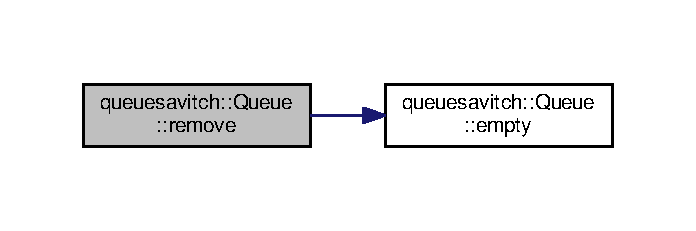
\includegraphics[width=334pt]{classqueuesavitch_1_1Queue_a607e9543f593526aee0d6a403a4ce775_cgraph}
\end{center}
\end{figure}




\subsection{Member Data Documentation}
\index{queuesavitch\+::\+Queue@{queuesavitch\+::\+Queue}!back@{back}}
\index{back@{back}!queuesavitch\+::\+Queue@{queuesavitch\+::\+Queue}}
\subsubsection[{\texorpdfstring{back}{back}}]{\setlength{\rightskip}{0pt plus 5cm}{\bf Queue\+Node\+Ptr} queuesavitch\+::\+Queue\+::back\hspace{0.3cm}{\ttfamily [protected]}}\hypertarget{classqueuesavitch_1_1Queue_a2759a808c5c9abe7d1c53cc8ade3f5a9}{}\label{classqueuesavitch_1_1Queue_a2759a808c5c9abe7d1c53cc8ade3f5a9}
\index{queuesavitch\+::\+Queue@{queuesavitch\+::\+Queue}!front@{front}}
\index{front@{front}!queuesavitch\+::\+Queue@{queuesavitch\+::\+Queue}}
\subsubsection[{\texorpdfstring{front}{front}}]{\setlength{\rightskip}{0pt plus 5cm}{\bf Queue\+Node\+Ptr} queuesavitch\+::\+Queue\+::front\hspace{0.3cm}{\ttfamily [protected]}}\hypertarget{classqueuesavitch_1_1Queue_ac30555d398c28ad9b72f9d9b05c1ddf6}{}\label{classqueuesavitch_1_1Queue_ac30555d398c28ad9b72f9d9b05c1ddf6}


The documentation for this class was generated from the following files\+:\begin{DoxyCompactItemize}
\item 
\hyperlink{Queue_8h}{Queue.\+h}\item 
\hyperlink{Queue_8cpp}{Queue.\+cpp}\end{DoxyCompactItemize}

\hypertarget{structqueuesavitch_1_1QueueNode}{}\section{queuesavitch\+:\+:Queue\+Node Struct Reference}
\label{structqueuesavitch_1_1QueueNode}\index{queuesavitch\+::\+Queue\+Node@{queuesavitch\+::\+Queue\+Node}}


{\ttfamily \#include $<$Queue.\+h$>$}



Collaboration diagram for queuesavitch\+:\+:Queue\+Node\+:
\nopagebreak
\begin{figure}[H]
\begin{center}
\leavevmode
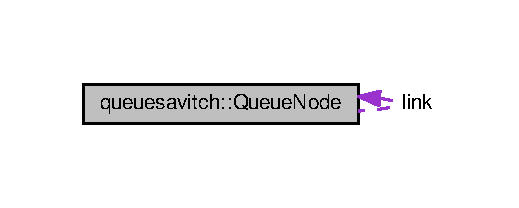
\includegraphics[width=249pt]{structqueuesavitch_1_1QueueNode__coll__graph}
\end{center}
\end{figure}
\subsection*{Public Attributes}
\begin{DoxyCompactItemize}
\item 
int \hyperlink{structqueuesavitch_1_1QueueNode_a4fd17a591c8510ed1118d3c4cb67b320}{data}
\item 
\hyperlink{structqueuesavitch_1_1QueueNode}{Queue\+Node} $\ast$ \hyperlink{structqueuesavitch_1_1QueueNode_add6ebeca47fc7ab55c99a33827cb68c4}{link}
\end{DoxyCompactItemize}


\subsection{Member Data Documentation}
\index{queuesavitch\+::\+Queue\+Node@{queuesavitch\+::\+Queue\+Node}!data@{data}}
\index{data@{data}!queuesavitch\+::\+Queue\+Node@{queuesavitch\+::\+Queue\+Node}}
\subsubsection[{\texorpdfstring{data}{data}}]{\setlength{\rightskip}{0pt plus 5cm}int queuesavitch\+::\+Queue\+Node\+::data}\hypertarget{structqueuesavitch_1_1QueueNode_a4fd17a591c8510ed1118d3c4cb67b320}{}\label{structqueuesavitch_1_1QueueNode_a4fd17a591c8510ed1118d3c4cb67b320}
\index{queuesavitch\+::\+Queue\+Node@{queuesavitch\+::\+Queue\+Node}!link@{link}}
\index{link@{link}!queuesavitch\+::\+Queue\+Node@{queuesavitch\+::\+Queue\+Node}}
\subsubsection[{\texorpdfstring{link}{link}}]{\setlength{\rightskip}{0pt plus 5cm}{\bf Queue\+Node}$\ast$ queuesavitch\+::\+Queue\+Node\+::link}\hypertarget{structqueuesavitch_1_1QueueNode_add6ebeca47fc7ab55c99a33827cb68c4}{}\label{structqueuesavitch_1_1QueueNode_add6ebeca47fc7ab55c99a33827cb68c4}


The documentation for this struct was generated from the following file\+:\begin{DoxyCompactItemize}
\item 
\hyperlink{Queue_8h}{Queue.\+h}\end{DoxyCompactItemize}

\chapter{File Documentation}
\hypertarget{PQmain_8cpp}{}\section{P\+Qmain.\+cpp File Reference}
\label{PQmain_8cpp}\index{P\+Qmain.\+cpp@{P\+Qmain.\+cpp}}
{\ttfamily \#include $<$iostream$>$}\\*
{\ttfamily \#include $<$cstdlib$>$}\\*
{\ttfamily \#include $<$cstddef$>$}\\*
{\ttfamily \#include \char`\"{}Queue.\+h\char`\"{}}\\*
{\ttfamily \#include \char`\"{}Priority\+Queue.\+h\char`\"{}}\\*
Include dependency graph for P\+Qmain.\+cpp\+:
\nopagebreak
\begin{figure}[H]
\begin{center}
\leavevmode
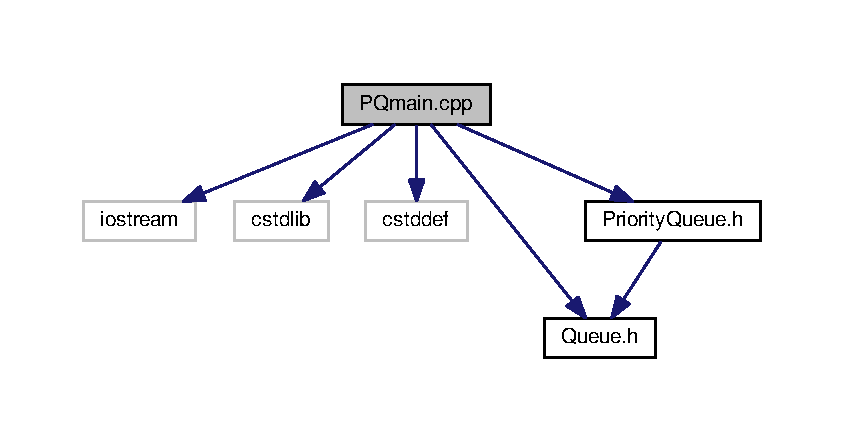
\includegraphics[width=350pt]{PQmain_8cpp__incl}
\end{center}
\end{figure}
\subsection*{Functions}
\begin{DoxyCompactItemize}
\item 
int \hyperlink{PQmain_8cpp_ae66f6b31b5ad750f1fe042a706a4e3d4}{main} ()
\end{DoxyCompactItemize}


\subsection{Function Documentation}
\index{P\+Qmain.\+cpp@{P\+Qmain.\+cpp}!main@{main}}
\index{main@{main}!P\+Qmain.\+cpp@{P\+Qmain.\+cpp}}
\subsubsection[{\texorpdfstring{main()}{main()}}]{\setlength{\rightskip}{0pt plus 5cm}int main (
\begin{DoxyParamCaption}
{}
\end{DoxyParamCaption}
)}\hypertarget{PQmain_8cpp_ae66f6b31b5ad750f1fe042a706a4e3d4}{}\label{PQmain_8cpp_ae66f6b31b5ad750f1fe042a706a4e3d4}

\begin{DoxyCode}
14 \{
15    \hyperlink{classqueuesavitch_1_1Queue}{Queue} q;
16    q.\hyperlink{classqueuesavitch_1_1Queue_a5f208f5455b566a5ddf3bb4a7869cb31}{add}(3);
17    q.\hyperlink{classqueuesavitch_1_1Queue_a5f208f5455b566a5ddf3bb4a7869cb31}{add}(9);
18    q.\hyperlink{classqueuesavitch_1_1Queue_a5f208f5455b566a5ddf3bb4a7869cb31}{add}(72);
19    q.\hyperlink{classqueuesavitch_1_1Queue_a5f208f5455b566a5ddf3bb4a7869cb31}{add}(825);
20    q.\hyperlink{classqueuesavitch_1_1Queue_a5f208f5455b566a5ddf3bb4a7869cb31}{add}(0);
21    q.\hyperlink{classqueuesavitch_1_1Queue_a5f208f5455b566a5ddf3bb4a7869cb31}{add}(52);
22 
23    cout << \textcolor{stringliteral}{"A queue filled with random numbers: \(\backslash\)n"};
24    cout << q.\hyperlink{classqueuesavitch_1_1Queue_a607e9543f593526aee0d6a403a4ce775}{remove}() << endl;
25    cout << q.\hyperlink{classqueuesavitch_1_1Queue_a607e9543f593526aee0d6a403a4ce775}{remove}() << endl;
26    cout << q.\hyperlink{classqueuesavitch_1_1Queue_a607e9543f593526aee0d6a403a4ce775}{remove}() << endl;
27    cout << q.\hyperlink{classqueuesavitch_1_1Queue_a607e9543f593526aee0d6a403a4ce775}{remove}() << endl;
28    cout << q.\hyperlink{classqueuesavitch_1_1Queue_a607e9543f593526aee0d6a403a4ce775}{remove}() << endl;
29    cout << q.\hyperlink{classqueuesavitch_1_1Queue_a607e9543f593526aee0d6a403a4ce775}{remove}() << endl;
30 
31    \hyperlink{classqueuesavitch_1_1PriorityQueue}{PriorityQueue} pq;
32    pq.\hyperlink{classqueuesavitch_1_1Queue_a5f208f5455b566a5ddf3bb4a7869cb31}{add}(3);
33    pq.\hyperlink{classqueuesavitch_1_1Queue_a5f208f5455b566a5ddf3bb4a7869cb31}{add}(9);
34    pq.\hyperlink{classqueuesavitch_1_1Queue_a5f208f5455b566a5ddf3bb4a7869cb31}{add}(72);
35    pq.\hyperlink{classqueuesavitch_1_1Queue_a5f208f5455b566a5ddf3bb4a7869cb31}{add}(825);
36    pq.\hyperlink{classqueuesavitch_1_1Queue_a5f208f5455b566a5ddf3bb4a7869cb31}{add}(0);
37    pq.\hyperlink{classqueuesavitch_1_1Queue_a5f208f5455b566a5ddf3bb4a7869cb31}{add}(52);
38 
39    cout << endl << \textcolor{stringliteral}{"A priority queue filled with the same numbers: \(\backslash\)n"};
40    cout << pq.\hyperlink{classqueuesavitch_1_1PriorityQueue_aabec9a46c41b0601f05f55a7894d20e1}{remove}() << endl;
41    cout << pq.\hyperlink{classqueuesavitch_1_1PriorityQueue_aabec9a46c41b0601f05f55a7894d20e1}{remove}() << endl;
42    cout << pq.\hyperlink{classqueuesavitch_1_1PriorityQueue_aabec9a46c41b0601f05f55a7894d20e1}{remove}() << endl;
43    cout << pq.\hyperlink{classqueuesavitch_1_1PriorityQueue_aabec9a46c41b0601f05f55a7894d20e1}{remove}() << endl;
44    cout << pq.\hyperlink{classqueuesavitch_1_1PriorityQueue_aabec9a46c41b0601f05f55a7894d20e1}{remove}() << endl;
45    cout << pq.\hyperlink{classqueuesavitch_1_1PriorityQueue_aabec9a46c41b0601f05f55a7894d20e1}{remove}() << endl;
46 
47    \textcolor{keywordflow}{return} 0;
48 \}
\end{DoxyCode}


Here is the call graph for this function\+:
\nopagebreak
\begin{figure}[H]
\begin{center}
\leavevmode
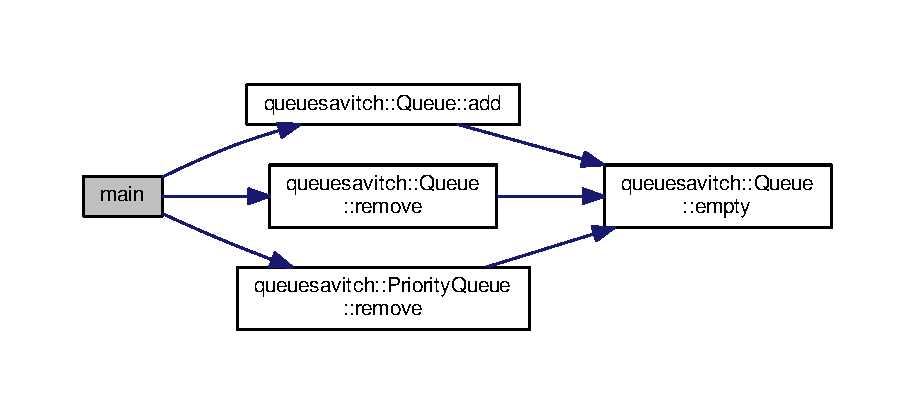
\includegraphics[width=350pt]{PQmain_8cpp_ae66f6b31b5ad750f1fe042a706a4e3d4_cgraph}
\end{center}
\end{figure}



\hypertarget{PriorityQueue_8cpp}{}\section{Priority\+Queue.\+cpp File Reference}
\label{PriorityQueue_8cpp}\index{Priority\+Queue.\+cpp@{Priority\+Queue.\+cpp}}
{\ttfamily \#include $<$iostream$>$}\\*
{\ttfamily \#include $<$cstdlib$>$}\\*
{\ttfamily \#include $<$cstddef$>$}\\*
{\ttfamily \#include \char`\"{}Queue.\+h\char`\"{}}\\*
{\ttfamily \#include \char`\"{}Priority\+Queue.\+h\char`\"{}}\\*
Include dependency graph for Priority\+Queue.\+cpp\+:
\nopagebreak
\begin{figure}[H]
\begin{center}
\leavevmode
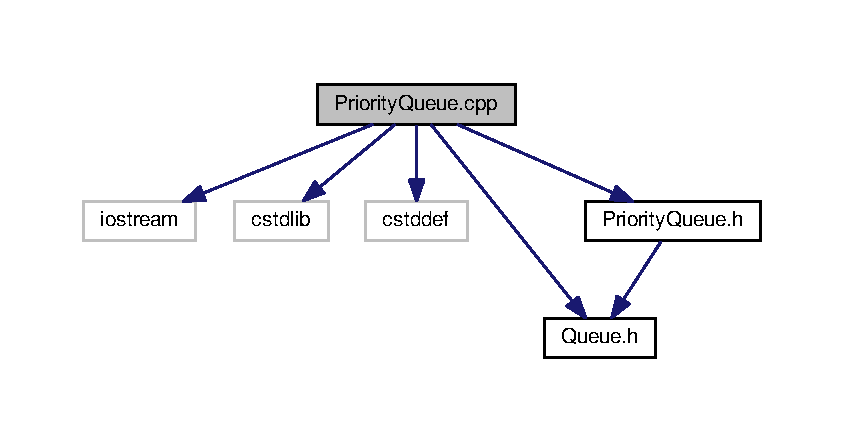
\includegraphics[width=350pt]{PriorityQueue_8cpp__incl}
\end{center}
\end{figure}
\subsection*{Namespaces}
\begin{DoxyCompactItemize}
\item 
 \hyperlink{namespacequeuesavitch}{queuesavitch}
\end{DoxyCompactItemize}

\hypertarget{PriorityQueue_8h}{}\section{Priority\+Queue.\+h File Reference}
\label{PriorityQueue_8h}\index{Priority\+Queue.\+h@{Priority\+Queue.\+h}}
{\ttfamily \#include \char`\"{}Queue.\+h\char`\"{}}\\*
Include dependency graph for Priority\+Queue.\+h\+:
\nopagebreak
\begin{figure}[H]
\begin{center}
\leavevmode
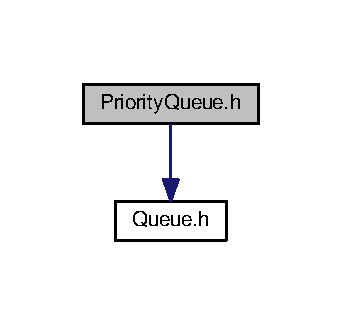
\includegraphics[width=164pt]{PriorityQueue_8h__incl}
\end{center}
\end{figure}
This graph shows which files directly or indirectly include this file\+:
\nopagebreak
\begin{figure}[H]
\begin{center}
\leavevmode
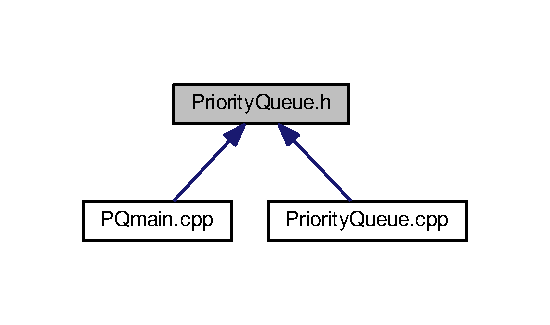
\includegraphics[width=264pt]{PriorityQueue_8h__dep__incl}
\end{center}
\end{figure}
\subsection*{Classes}
\begin{DoxyCompactItemize}
\item 
class \hyperlink{classqueuesavitch_1_1PriorityQueue}{queuesavitch\+::\+Priority\+Queue}
\end{DoxyCompactItemize}
\subsection*{Namespaces}
\begin{DoxyCompactItemize}
\item 
 \hyperlink{namespacequeuesavitch}{queuesavitch}
\end{DoxyCompactItemize}

\hypertarget{Queue_8cpp}{}\section{Queue.\+cpp File Reference}
\label{Queue_8cpp}\index{Queue.\+cpp@{Queue.\+cpp}}
{\ttfamily \#include $<$iostream$>$}\\*
{\ttfamily \#include $<$cstdlib$>$}\\*
{\ttfamily \#include $<$cstddef$>$}\\*
{\ttfamily \#include \char`\"{}Queue.\+h\char`\"{}}\\*
Include dependency graph for Queue.\+cpp\+:
\nopagebreak
\begin{figure}[H]
\begin{center}
\leavevmode
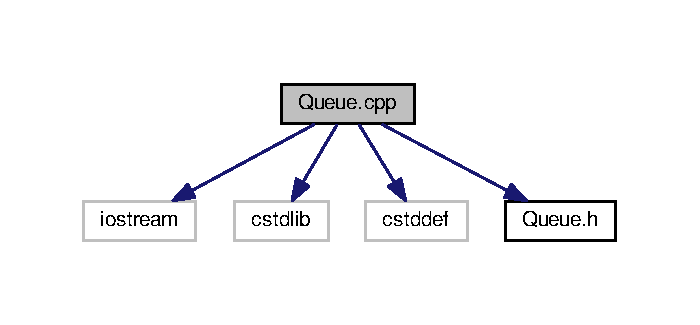
\includegraphics[width=336pt]{Queue_8cpp__incl}
\end{center}
\end{figure}
\subsection*{Namespaces}
\begin{DoxyCompactItemize}
\item 
 \hyperlink{namespacequeuesavitch}{queuesavitch}
\end{DoxyCompactItemize}

\hypertarget{Queue_8h}{}\section{Queue.\+h File Reference}
\label{Queue_8h}\index{Queue.\+h@{Queue.\+h}}
This graph shows which files directly or indirectly include this file\+:
\nopagebreak
\begin{figure}[H]
\begin{center}
\leavevmode
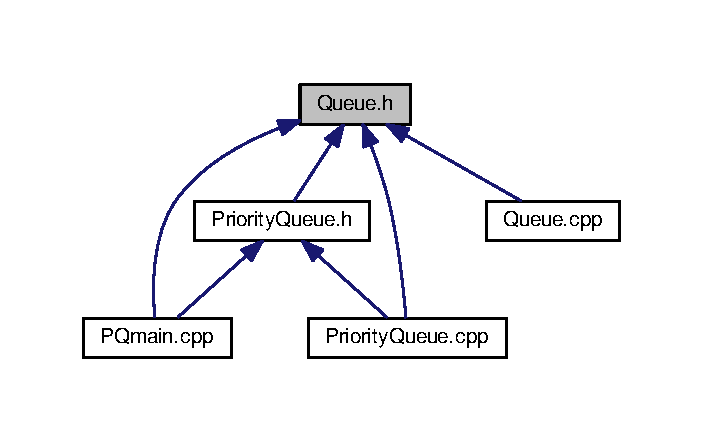
\includegraphics[width=338pt]{Queue_8h__dep__incl}
\end{center}
\end{figure}
\subsection*{Classes}
\begin{DoxyCompactItemize}
\item 
struct \hyperlink{structqueuesavitch_1_1QueueNode}{queuesavitch\+::\+Queue\+Node}
\item 
class \hyperlink{classqueuesavitch_1_1Queue}{queuesavitch\+::\+Queue}
\end{DoxyCompactItemize}
\subsection*{Namespaces}
\begin{DoxyCompactItemize}
\item 
 \hyperlink{namespacequeuesavitch}{queuesavitch}
\end{DoxyCompactItemize}
\subsection*{Typedefs}
\begin{DoxyCompactItemize}
\item 
typedef Queue\+Node $\ast$ \hyperlink{namespacequeuesavitch_a3a9d48cafb7ea2049936da3b05a10209}{queuesavitch\+::\+Queue\+Node\+Ptr}
\end{DoxyCompactItemize}

%--- End generated contents ---

% Index
\backmatter
\newpage
\phantomsection
\clearemptydoublepage
\addcontentsline{toc}{chapter}{Index}
\printindex

\end{document}
